\section{Реализация решения}\label{chapter3}

В главе \ref{chapter2} было представлено описание решения, которое позволит получить промежуточные состояния потока объектов между вызовами операций Stream API. Чтобы применить решение на практике, реализуем расширение для среды разработки IntelliJ IDEA. 

IntelliJ IDEA -- среда для разработки, основанная на платформе IntelliJ, позволяет разрабатывать программы на нескольких языках программирования, в том числе на java. Функциональность платформы может быть расширена с помощью плагинов, которые могут быть установлены из официального репозитория \cite{jb:plugins}, либо из других источников. Платформа предоставляет разработчикам плагинов API -- классы и интерфейсы, с помощью которых компоненты плагина могут быть интегрированы в работу платформы.
\subsection{Нахождение подходящего вызова}

Для нахождения границ вызова будем использовать API, предоставляемый платформой для работы с исходным кодом. Исходный код представляется в виде $AST$ (абстрактное синтаксическое дерево \cite{wiki:ast}). Обходя его, можно найти цепочки вызовов. Интерфейс платформы позволяет определить тип объекта, на котором вызывается метод и тип результата вызова. Используя следующие правила, мы сможем классифицировать вызовы внутри цепочки:
\begin{itemize}
	\item Промежуточный вызов -- возвращает объект, реализующий \mintinline{java}{Stream<T>}.
	\item Завершающий вызов - происходит на объекте, реализующем \mintinline{java}{Stream<T>}, возвращает объект произвольного типа, который не реализует \mintinline{java}{Stream<T>}. 
\end{itemize}

Учитывая, что положение отладчика может быть отображено на некоторый элемент $AST$, у нас есть возможность обойти поддерево этого элемента и найти все подходящие цепочки. Кроме того, мы не привязываемся к именам методов для промежуточных операций, это снижает требование к потоку, который может быть отлажен (вызовы с неподдерживаемым операциями могут отлаживаться: для них будут построены состояния, но переходы восстановить не удастся). Таким образом, можно удовлетворить всем требованиям из \ref{detection}.

Отдельно стоит рассмотреть редкий случай, когда результат завершающей операции наследник \mintinline{java}{Stream<T>}. Действуя неосторожно, можно перепутать такую завершающую операцию с промежуточной. Чтобы этого избежать, необходимо проверить, что имя промежуточной операции не совпадает с именами терминальных операций, которые могут вернуть \mintinline{java}{Stream<T>}. Таких операций немного -- \mintinline{java}{collect} и \mintinline{java}{reduce}.

\subsection{Построение выражения} 
Во второй главе был получен важный результат. Для того, чтобы восстановить все переходы, их нужно восстановить локально для каждого из промежуточных вызовов. При этом необходимая информация для построения переходов у разных операций может различаться. Поэтому будет удобно ввести абстракции, которые позволят каждому вызову модифицировать цепочку, чтобы собрать данные для восстановления переходов. 

Для всех вызовов верно, что они требуют лишь локальной модификации цепочки: добавления методов до и после самого вызова. 

Таким образом, достаточно ввести абстракции, которые позволят:
\begin{itemize}
	\item Объявлять локальные переменные, нужные для сохранения информации о вычислении, в выражении для вычисления.
	\item Добавлять промежуточные вызовы в цепочку до и после самой операции.
	\item Преобразовывать собранную информацию в процессе запуска выражения к удобному представлению для дальнейшей интерпретации.
\end{itemize}

При этом нужно позаботиться, чтобы имена локальных переменных, которые используют разные вызовы были различны. Самый простой способ этого достичь -- добавить к имени используемых переменных порядковый номер вызова в исходной цепочке.

Структура фрагмента кода для вычисления, с точки зрения одной операции, будет выглядеть следующим образом:

\inputminted{java}{chapter3/code/EvalCode.java}

В примере выше показано, как вызов, для которого мы хотим построить состояния и переходы, может воспринимать структуру генерируемого кода. Этот вызов является $K$-м по порядку в цепочке из $M$ методов. Его основные особенности:
\begin{itemize}
	\item Массив \mintinline{java}{trace} используется для сохранения результатов. Имеено он является результатом вычисления фрагмента этого фрагмента кода.
	\item В начале фрагмента происходит определение всех переменных, использующихся для сбора данных о объектах внутри потока. Различным вызовам может требоваться разное количество переменных.
	\item После определения переменных расположен вызов модифицированной цепочки. Каждая операция исходной цепочки дополнила её требуемыми вызовами до и после самой операции. Количество этих вызовов определяется потребностями вызова.
	\item После каждого вызова исходной цепочки добавлен вспомогательный вызов \mintinline{java}{peek}. Его цель -- увеличить глобальное время (\ref{build-expression}) после появления нового объекта в цепочке. 
	\item Затем последовательно заполняется массив \mintinline{java}{trace}. Исходные значения переменных могут быть неудобными для интерпретации, поэтому их стоит трансформировать так, чтобы на стороне IDE, этими данными было удобно оперировать (см \ref{impl:interpter}). Обычно это означает конвертацию вспомогательных значений в массивы (возможно, вложенные).
\end{itemize}

Пример сгенерированного кода есть в приложении А.

\subsection{Вычисление выражения}
В \ref{code-evaluation} описаны подходы к вычислению произвольного кода внутри отладчика. Там же был сделан выбор в пользу стратегии загрузки и запуска новых классов. Данная возможность уже присутствует в среде разработки, поэтому не будем подробно останавливаться на деталях реализации этого процесса. У такого подхода есть недостаток -- у загружаемых классов может не быть прав доступа к некоторым полям и методам других объектов. Это происходит из-за того, что новый класс компилируется как внутренний класс для класса, внутри которого находится отладчик при запуске операции вычисления выражения. Но класс, в котором находится отладчик уже загружен, и он не знает о новом внутреннем классе, поэтому не может предоставить доступ к приватным полям и методам.

Для решения этой проблемы используется внутренний класс JDK \\ \mintinline{java}{MagicAccessorImpl} \cite{magic}. Это часть небезопасного API java. Наследование от этого класса является указанием для виртуальной машины java, что необходимо пропускать проверки доступа при вызове методов и обращении к полям из методов класса-наследника \mintinline{java}{MagicAccessorImpl}.

Кроме сгенерированного класса, анонимные функции тоже могут пытаться получить доступ к приватным методам и полям. В текущей версии платформы это приведет к исключению. Но это можно обойти, преобразовав все анонимные функции, которые встречаются в выражении, в анонимные классы, которые наследуются от \mintinline{java}{MagicAccessorImpl}. Для этого преобразования можно использовать существующие рефакторинги для преобразования анонимных функций в анонимные классы.

Таким образом, весь код внутри выражения для построения состояний и переходов не будет иметь проблем с доступом к методам и полям других классов.

\subsection{Интерпретация результата вычисления выражения}  \label{impl:interpter}
В \ref{state-transitions-build} был предложен способ восстановления переходов по информации, собранной на этапе вычисления выражения. Результатом вычисления является некий объект, в котором хранится вся собранная информация. Для упрощения обработки этой информации потребуем, чтобы она хранилась только в массивах. Это обусловлено тем, что JDI позволяет получить элементы массива без вызова дополнительных методов на отлаживаемой виртуальной машине. Заметим, что вспомогательные значения и объекты, которые использовались для сохранения информации при вычислении, всегда можно представить как массив объектов:
\begin{itemize}
	\item Если этот объект был типа \mintinline{java}{Map<Key, Value>}, то его можно представить в виде двух массивов: массив ключей и массив значений. Сами ключи и значения, в свою очередь, так же могут быть массивами.
	\item Другие коллекции очевидным образом могут быть представлены в виде массивов.
	\item Произвольный объект \mintinline{java}{reference} может быть сохранен в виде массива: \\ \mintinline{java}{new Object[] {reference}}.
	\item Значение примитивного типа, тоже может быть обернуто в массив. Например, так \mintinline{java}{new int[] {42}}.
\end{itemize}

Эти преобразования нужно выполнять только для вспомогательных структур данных. Для объектов из потока этого делать не нужно.

В результате интерпретации и разрешения переходов согласно правилам из \ref{interpret}, получим промежуточные состояния и переходы объектов между соседними состояниями.

\subsection{Визуализация}
После завершения этапа интерпретации имеется набор промежуточных состояний и переходы между ними. Промежуточные состояния -- это просто список объектов. Переходы -- это связь между объектам в двух соседних состояниях. Наиболее естественно это визуализировать с помощью двух списков объектов и линий-переходов.

При выборе какого-либо значения в списке нужно визуально выделить все объекты из соседних состояний, с которыми он связан переходами, затем те, с которыми связаны они и так далее. 
\newpage
В результате пользовательский интерфейс имеет следующий вид:

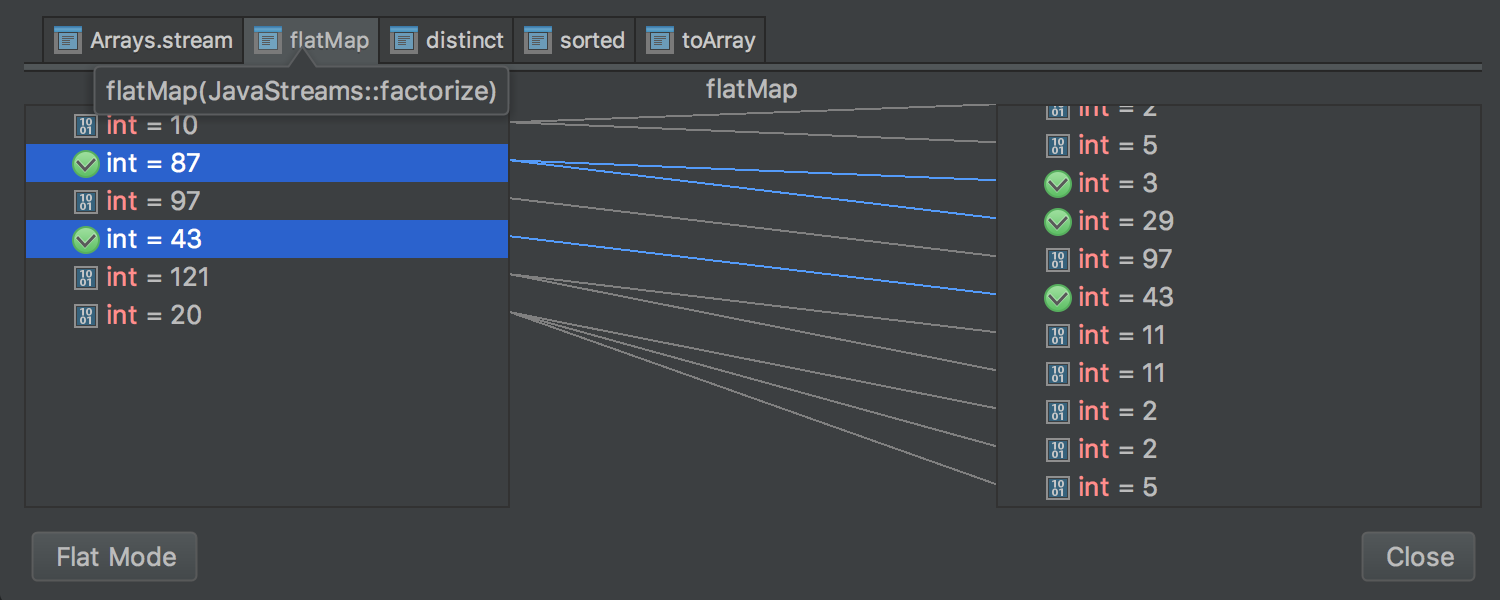
\includegraphics[scale=0.3]{chapter3/img/split-view.png}

Дополнительно, есть возможность просмотреть всю цепочку целиком:

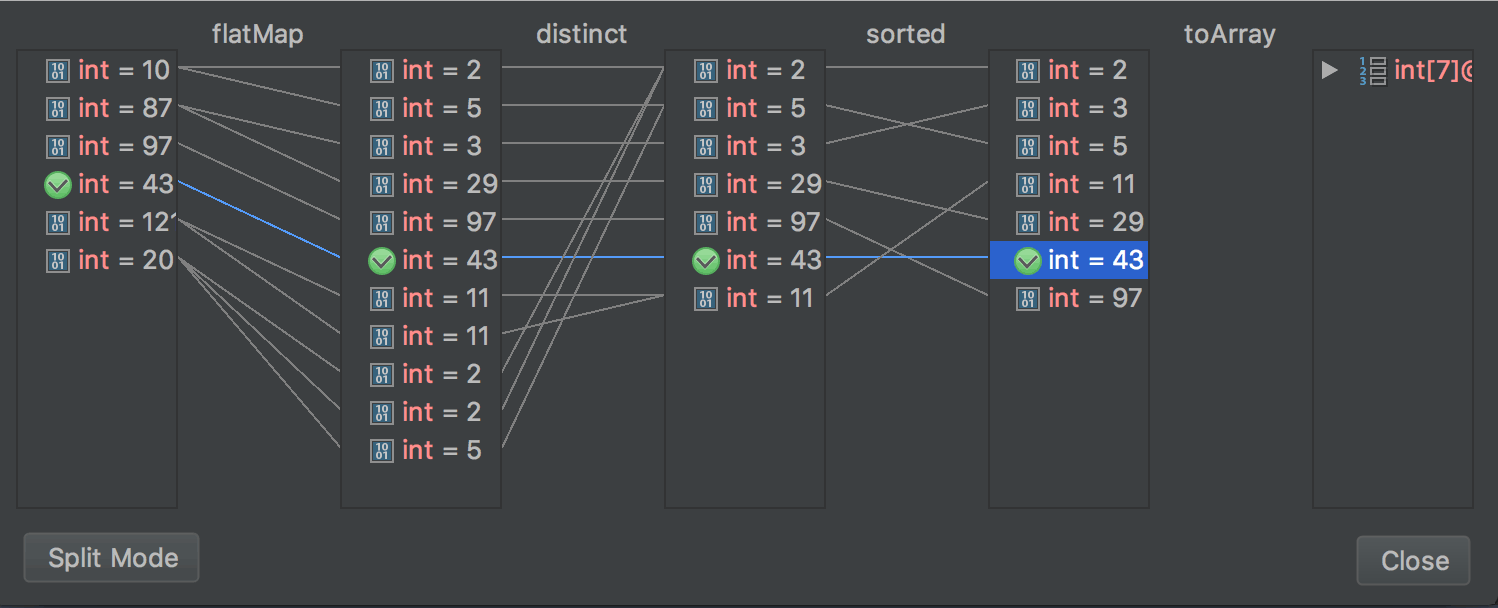
\includegraphics[scale=0.4]{chapter3/img/flat-view.png}










